\chapter{Introduction}
% Fill with what you want to include in the introduction
\epigraph{``Simplicity is a great virtue but it requires hard work to achieve it and education to appreciate it. And to make matters worse: complexity sells better.''}{\textit{Edsger W. Dijkstra}}

\section*{What is an ISA?}

A computer is a device which is capable of acquiring data, performing calculations upon it, and making the results available for use at a later date.
It is clear from this definition, that when deciding how to design and build a computer one must at least take into consideration the way data is 
stored and organized (the memory) and the mechanisms through which the computer is able to manipulate said data (the processor).
Computers are an abstract concept and do not impose a certain technological choice to their physical realization. Nonetheless, the vast majority of computers nowadays
are built through the assembly of digital components and thus natively speak the language of the binary number system.
As such, just like when using a mechanical device an operator needs to interact with the physical parts of the system,  operating a computer at this level
would require the user to manually insert ones and zeros into the right places for it to perform its calculations.
It is clear that such an operation would require an intimate knowledge of the physical implementation of the computer, and even minimal
changes to its digital circuitry might jeopardize the correctness of any sequences of bits written for an earlier model.

Early on in the history of computers it was understood that an additional layer of abstraction was needed in order to separate the hardware from the software
and give more freedom both to the circuit designers and the programmers. This layer of abstraction is called an Instruction Set Architecture,
which from now on will be called ISA for short. An ISA provides a logical specification of how a computer manages its memory and what the instructions that it's
capable of performing are. This forms the layer through which all software must interface with in order to interact with the hardware.

\section*{What is the LEGv8 ISA?}

The ISA focus of this thesis is the LEGv8 ISA, an ARM-inspired architecture created by David A. Patterson and John L. Hennessy designed to serve as a teaching
tool in their book \emph{Computer Organization and Design (ARM Edition)}. As the title suggests, the book is actually about the ARMv8 ISA, whose first
iteration was originally released in 1983 by Acorn Computers and which is now developed by Arm Holdings plc. The authors, however, have introduced a few
changes and simplifications to the ARMv8 ISA to make it friendlier to students and emphasize certain design concepts. As such, this ISA is used
in the sections of the book dedicated to the design of a model processor and its programming, and it's these sections upon which the LEGv8 simulator
subject of this thesis is based.

\section*{Overview of the LEGv8 ISA}

\begin{figure}[H]
	\centering
	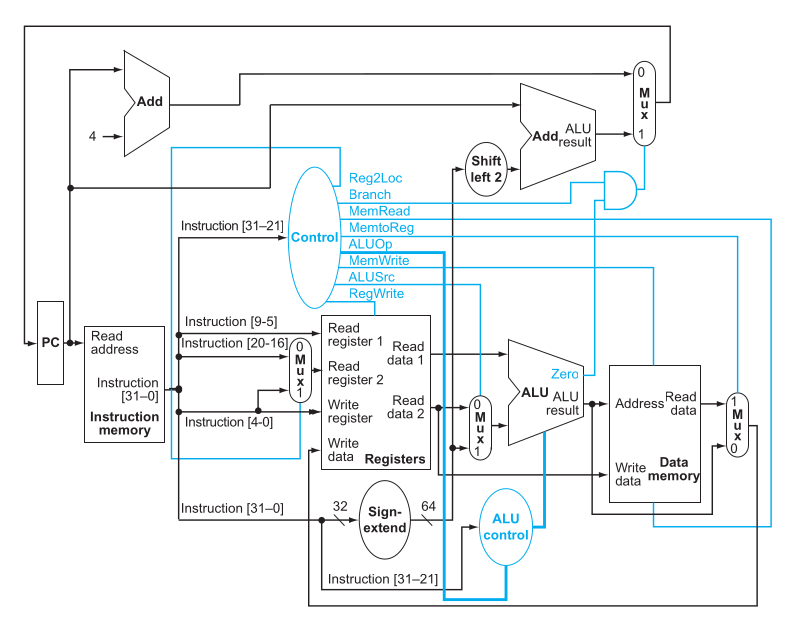
\includegraphics[width=.8\textwidth]{img/legv8_logical_scheme.png}
	\caption{The logical scheme of the LEGv8 architecture}
\end{figure}

\subsection*{Architecture type}
LEGv8 follows the Von Neumann architecture paradigm and thus contemplates the existence of a single memory containing both the instructions and the program data. It is a 64-bit architecture and is specifically designed for pipelined execution.
\subsection*{Registers}
LEGv8 defines 32 64-bit \emph{X} registers for storing integer values and 32 64-bit \emph{D} registers for storing double precision floating point values. There are also 32 32-bit \emph{S} registers dedicated to single precision floating point values, albeit being purely logical and simply occupying the lower 32 bits of the \emph{D} registers. Unlike ARMv8, the presence of 32-bit \emph{W} integer registers is not contemplated.
\newline
Registers are also used following a certain convention that is defined by the ISA but not enforced by the processor, and some can be addressed using alternative names for readibility purposes. There are analogous conventions for floating point registers too.
\begin{figure}[H]
	\centering
	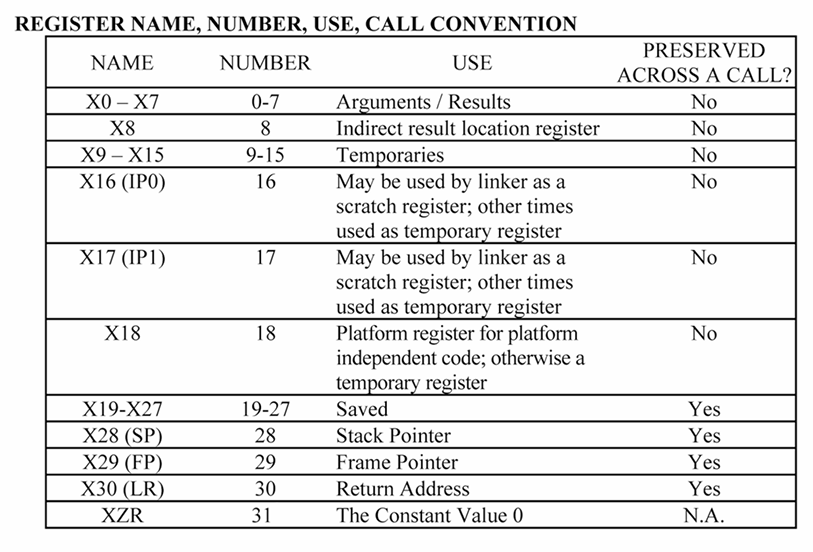
\includegraphics[width=.8\textwidth]{img/registers_conventions.png}
	\caption{Integer registers usage convention}
\end{figure}
\newline

In addition to the normal registers directly accessible by the programmer, more exist to store the program counter (i.e. the address of the current instruction to be executed) and various flags to keep track of overflows or carry bits in arithmetic operations and comparisons.
\subsection*{Memory}
The memory contains both the program code and the data. It is logically divided into a \emph{reserved} segment, a \emph{text} segment containing the program code, a \emph{static data} segment containing the constants defined at compile time, and a \emph{dynamic data} and \emph{stack} segments occupying the same location of memory and respectively growing upwards from the \emph{static data} segment and downwards from the stack pointer. This section of the memory is the one containing the data defined at execution time.
\begin{figure}[H]
	\centering
	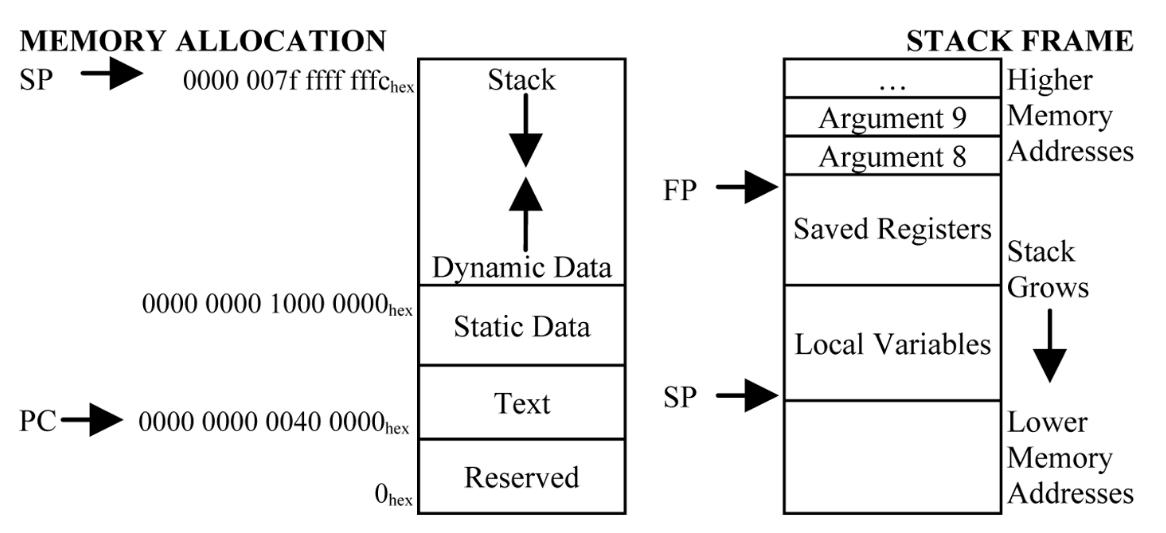
\includegraphics[width=.8\textwidth]{img/main_memory_layout.png}
	\caption{Logical division of the memory}
\end{figure}
\subsection*{Control unit}
The control unit is the component responsible for coordinating the pipeline execution flow and configuring the various components to perform the desired operations in the correct order using the correct parameters.
\subsection*{ALU}
The LEGv8 ALU is capable of performing 64-bit integer operations and both single and double precision floating point operations. The operation to perform at any given moment is configured through an ALUop code provided by the control unit.
\subsection*{Pipeline}
The LEGv8 pipeline is comprised of 5 stages: \emph{fetch}, \emph{decode}, \emph{execute}, \emph{data access}, and \emph{write back}.
As the names suggest, the \emph{fetch} stage is responsible for acquiring instructions from the text segment of the memory, the \emph{decode} stage decodes the instructions, reads the registers involved in the operation, and configures the control unit accordingly, the \emph{execute} stage performs the calculation through the ALU, the \emph{data access} stage is responsible for accessing the the memory, and the \emph{write back} stage finally writes the result into the registers.
Of course not all instructions make use of all the pipeline stages and this is taken into consideration when optimizing the execution flow.
\begin{figure}[H]
	\centering
	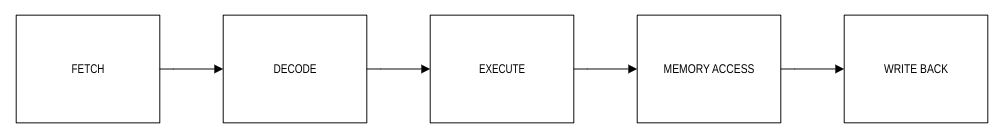
\includegraphics[width=.8\textwidth]{img/5_stage_pipeline.png}
	\caption{The 5 pipeline stages}
\end{figure}
\subsection*{Instructions}
LEGv8 can be considered a subset of ARMv8, but with a few caveats. Many higher level instructions have been omitted altogether in order to keep the ISA as minimal as possible, and many of the ones that have been kept have been revisited to make them clearer in their scope. For example, in ARMv8 the \emph{ADD} instruction can be used with both 32 and 64 bit integer registers, and both with register-based and immediate-based (i.e. defined directly in the program code) values. This of course allows the ARMv8 programmer to remember a single mnemonic and use it in all sorts of operations, but it obscures some important underlying design differences that might be valuable to computer architecture students. In LEGv8 instead, it has been decided to split the \emph{ADD} instruction into \emph{ADD} and \emph{ADDI} or register and immediate values usage respectively. Similarly, in ARMv8 the \emph{FADD} instruction is capable of performing additions both in the case of single and double precision registers, whereas in LEGv8 the instruction has been split into \emph{FADDS} and \emph{FADDD} for performing the operation only on single precision or double precision registers respectively.
\begin{figure}[H]
	\centering
	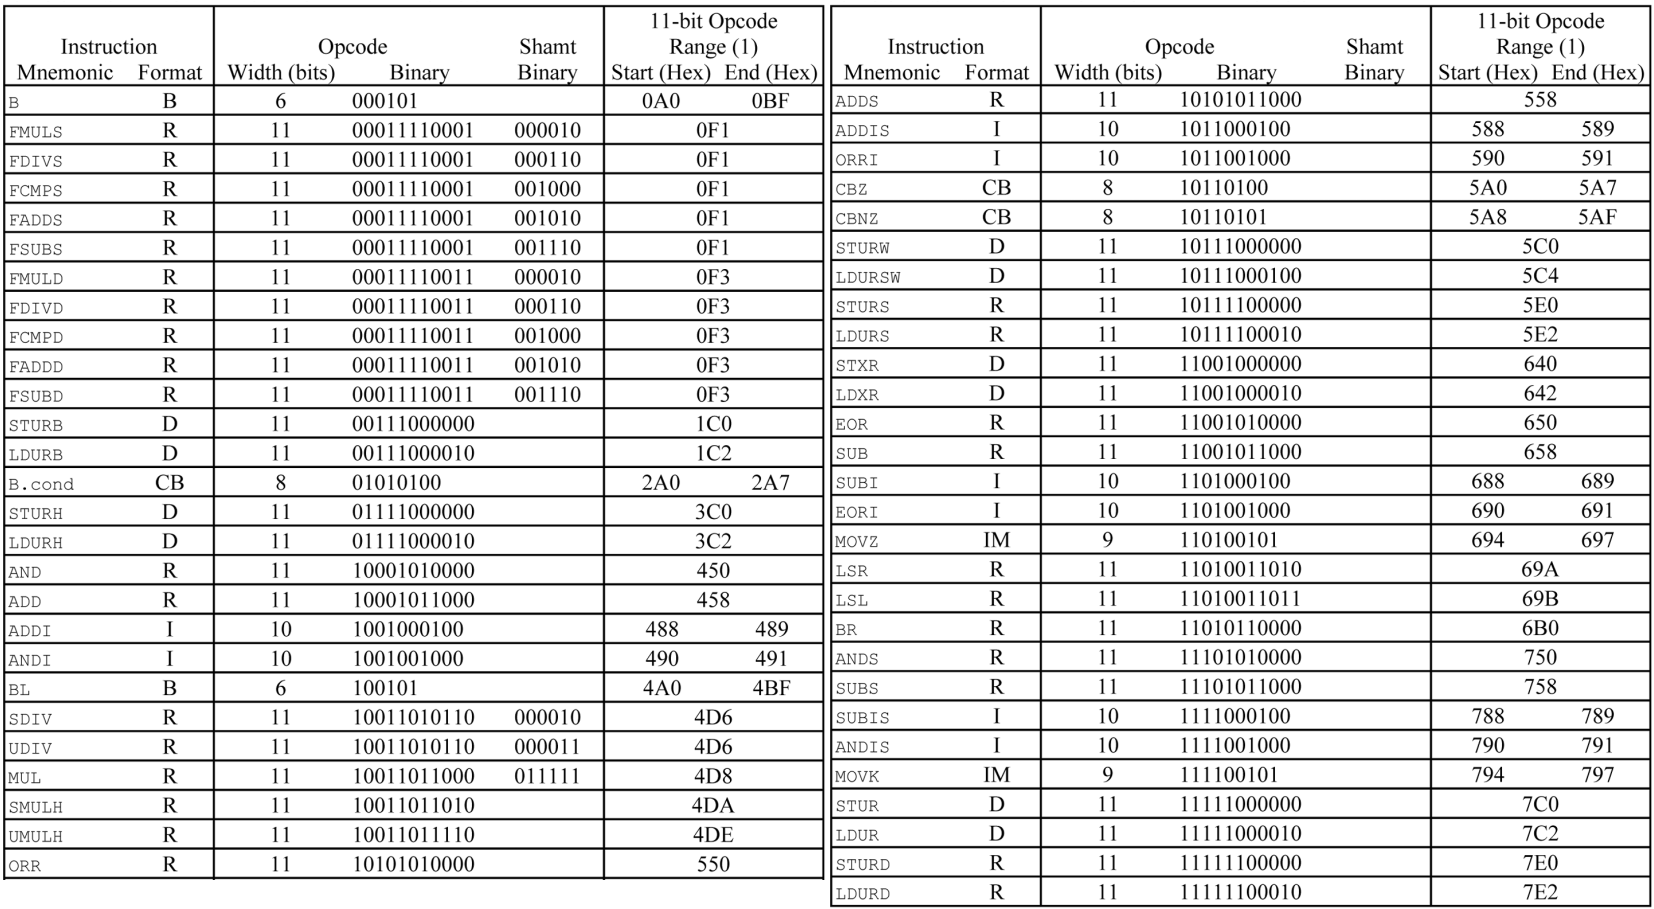
\includegraphics[width=.8\textwidth]{img/legv8_instruction_set.png}
	\caption{The complete LEGv8 ISA}
\end{figure}
All the instructions are encoded with the same length of 32 bits in order to fetch and decode them more efficiently. They are also grouped into 5 instruction formats to give a more homogeneous encoding to operations performing similar steps and increase their decoding speed.
The \emph{R}-type instructions perform operations solely on registers, the \emph{I}-type instructions make use of immediate values, the \emph{D}-type instructions access the memory, the \emph{B}-type and \emph{CB} perform unconditional and conditional branching respectively, and the \emph{IW}-type instructions to perform MOV instructions with wider immediate values.
\begin{figure}[H]
	\centering
	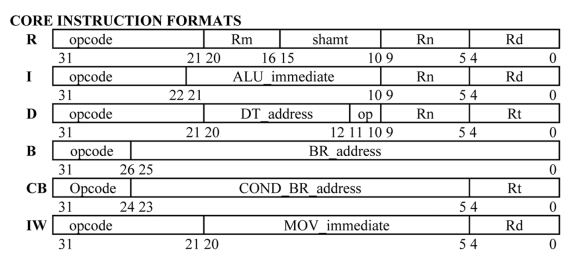
\includegraphics[width=.8\textwidth]{img/instruction_types.png}
	\caption{The 5 formats of LEGv8 instructions with their encoding pattern}
\end{figure}
\section*{Motivations for choosing LEGv8}
The LEGv8 ISA, being presented and defined in one of the major computer architecture undergraduate textbooks, is taught in many university courses around the world, including the Digital Systems Architecture course held by Prof. Carini at UniTS. In spite of its popularity, no real hardware has been made to run its instruction set natively, and the simulator landscape is almost equally lacking in viable options. This in turn makes it impossible for educators and students alike to show working examples of LEGv8 code, depriving them of teaching and learning opportunities. For these reasons I have chosen to work on an already existing and partially working LEGv8 simulator provided by Arm Holdings plc. to expand upon its functionalities to include a complete simulation of the ISA. 


